
\documentclass[preprint,12pt]{elsarticle}

\usepackage{amssymb}
\usepackage{amsmath,dsfont}
\usepackage{amsthm}
\usepackage[ruled,vlined, linesnumbered]{algorithm2e}
\usepackage{pgfplots}
\usepackage[utf8]{inputenc}
\usepackage{url}
\usepackage{tikz}
\usepackage{caption}
\usepackage{subfig}
\tikzset{
  font={\fontsize{9pt}{12}\selectfont}}
\newtheorem{theorem}{Theorem}[section]
\newtheorem{lemma}[theorem]{Lemma}
\newtheorem{proposition}[theorem]{Proposition}
\newtheorem{corollary}[theorem]{Corollary}
\newcommand{\R}{\mathbb{R}}
\newcommand{\N}{\mathbb{N}}
\DeclareMathOperator*{\argmin}{arg\,min}
\definecolor{gr}{HTML}{00BB00}
\setlength\parindent{0pt}

\journal{European Journal of Operational Research}

\begin{document}

\begin{frontmatter}

%% Title, authors and addresses

%% use the tnoteref command within \title for footnotes;
%% use the tnotetext command for theassociated footnote;
%% use the fnref command within \author or \address for footnotes;
%% use the fntext command for theassociated footnote;
%% use the corref command within \author for corresponding author footnotes;
%% use the cortext command for theassociated footnote;
%% use the ead command for the email address,
%% and the form \ead[url] for the home page:
%% \title{Title\tnoteref{label1}}
%% \tnotetext[label1]{}
%% \author{Name\corref{cor1}\fnref{label2}}
%% \ead{email address}
%% \ead[url]{home page}
%% \fntext[label2]{}
%% \cortext[cor1]{}
%% \address{Address\fnref{label3}}
%% \fntext[label3]{}

\title{Globally convergent decomposition algorithm for risk parity problem in portfolio selection}

%% use optional labels to link authors explicitly to addresses:
%% \author[label1,label2]{}
%% \address[label1]{}
%% \address[label2]{}

\author[mosek]{A.Cassioli\fnref{mail-cassioli}}
\author[firenze]{G.Cocchi\fnref{mail-cocchi}}
\author[firenze]{F.D'Amato\fnref{mail-damato}}
\author[firenze]{M.Sciandrone\fnref{mail-sciandrone}}

\address[mosek]{MOSEK ApS, Copenhagen, Denmark}
\address[firenze]{Dipartimento di Ingegneria dell'Informazione, Università di Firenze, Firenze, Italy}


\fntext[mail-cassioli]{andrea.cassioli@mosek.com}
\fntext[mail-cocchi]{guido.cocchi@unifi.it}
\fntext[mail-damato]{federico.damato@stud.unifi.it}
\fntext[mail-sciandrone]{marco.sciandrone@unifi.it}

\begin{abstract}
%% Text of abstract

\end{abstract}

\begin{keyword}
TODO\sep Portfolio\sep Risk-Parity \sep decomposition \sep optimization
%% keywords here, in the form: keyword \sep keyword

%% PACS codes here, in the form: \PACS code \sep code

%% MSC codes here, in the form: \MSC code \sep code
%% or \MSC[2008] code \sep code (2000 is the default)

\end{keyword}

\end{frontmatter}

%% \linenumbers

%% main text
\section{Introduction}
%%write something
The most important problem in budget allocation is making a good porfolio in terms of expected return and volatility. 
A lot of models were based on the Markowitz theory, stated in 1950s, for finding portfolio in the efficient frontier. 
All these approaches are proved to be unsuitable to real contexts, due to the market unstability and the ill-conditions of the problems. 
% aggiungere diversificazione
So the scientific community did a lot of works to find a way to minimize only the risk or the diversification. 
Many naive techniques as Equally Weighting (EW) portfolios were adopted in several real contexts showing poor perfomance, altought they have good theoretical performance. 
The Risk Parity concept was proposed in \cite{qian2005} to construct a portfolio such that all the asset contributions to the total risk are equal to each other \cite{maillard}.
Many different formulations were used to deal with Risk Parity, depending also on the absence of the \emph{short-selling} constraint (i.e. $x\ge0$).
In \cite{maillard} a nonlinear nonconvex least-squares optimization model without short-selling constraint was proposed.

In \cite{tardella2016} an equally bounded risk formulation was proposed, in which all the risk contributions are equally upper bounded by the same variable. It can be proved that an optimal solution for the long-short ERB is also a Risk Parity solution with minimum variance.
In \cite{feng2016} a scalarized version of a multi-objective optimization problem considering the expected return the risk the sparsity and the risk parity was addressed with a successive convex approximations.
In \cite{tutuncu} a lightly modification of the least-squares approach was proposed considering another optimization variable $\theta$ which represents the value around which all risk contribution will stay.
\begin{subequations}\label{eq:problemRP} 
\begin{align}
\min_{x,\theta} & \quad f(x,\theta) =  \sum_{i=i}^n \left(x_i(Q x)_i - \theta\right)^2 \\
\text{s.t.} & \quad l \leq x \leq u \\
& \quad \mathds{1}^T x = 1 
\end{align}
\end{subequations}
Due to its more readable form and its lower evaluating cost, we consider that formulation as our optimization problem.
Because of Sequential Quadratic Programming has poor performance when the number of assets increases, we proposed a globally convergent decomposition algorithm which uses a two level decomposition framework.
We use a Gauss-Seidel decomposition with respect to the two blocks $x,\theta$, then when we have to optimize the $x$ block we use a Gauss-Southwell decomposition which select the Most Violating Pair for the optimality conditions among all the asset variables. Then we decrease the objective function with a line search considering only the MVP pair.

The paper proceeds as follow: in section blablablabla.


\begin{proposition}
evbrfretre
\end{proposition}
\clearpage
\section{Preliminary background}\label{sect:2}
\input{preliminary_MS}
\clearpage
\section{A decomposition framework}
As already discussed, we partition the vector of variables into two blocks in order to take into account
the structure of the feasible set and possibly the form of the objective function (see, for instance,
the formulation of the risk parity problem, where the objective function is convex w.r.t. the scalar variable $\theta$).
The first block contains the constrained variables $x$, the second block contains
the unconstrained variables $y$. 

A first possibility can be that of defining a two-blocks Gauss-Seidel algorithm.
According to this scheme, at each iteration, the two component vectors $x$ and $y$ are
sequentially updated by performing  minimization steps (either exact or inexact) by  suitable descent techniques.
Globally convergent results of Gauss-Seidel algorithms (both exact and inexact) have been established in \cite{}, \cite{}, \cite{}.

We present here a block descent algorithm where a further level of decomposition is
introduced with respect to the block component $x$. 
More specifically, at each iteration, only two variables are updated, those corresponding
to a {\it Violating Pair}, by performing an inexact line search along a feasible and descent direction.
In order to guarantee convergence, the {\it Most Violating Pair} must be selected at least periodically, say every $M$ iterations.
We will discuss in the section of the computational experiments the role and the influence of the parameter $M$.

The adoption of a decomposition strategy with respect to the subvector $x$ is suitable
whenever the number $n$ of variables is large.

Note that the properties of the standard Armijo-type line search do not guarantee, without further assumptions
on the descent search direction $d^k$, that the distance between successive points tends to zero, which is a usual requirement of decomposition methods. 
This motivates the employment of the Quadratic Line Searck (QLS) defined in the appendix and based on the acceptance condition
$$
f((x^k,y^k)+\alpha^kd^k)\le f((x^k),y^k))-\gamma (\alpha^k)^2\|d^k\|^2.
$$
Concerning the unconstrained block component $y$, we do not specify the updating rule, but we state the following assumption that
could be satisfied, in practice, by different techniques depending on the hypothesis on $f$.
\par\medskip\noindent
{\bf Assumption on the updating rule of} $y$.
\par\medskip\noindent
\begin{itemize}
\item[(i)] For each $k$ we have $f(x^k,y^{k+1})\le f(x^k,y^k)$
\item [(ii)] If
$$
\lim_{k\to\infty} \left(f(x^k,y^{k+1})- f(x^k,y^k)\right)=0
$$
then
$$
\lim_{k\to\infty}\|y^{k+1}-y^k\|=0
$$
and
$$
\lim_{k\to\infty}\nabla_y f(x^k,y^k)=0.
$$
\end{itemize}


%At every step $k$ we choose a random subset $W^k\subset \{1,..,n\}$ such as
%\begin{equation}\label{eq:lambda}
%\frac{|W^k|}{n} \times 100 = \lambda
%\end{equation}
%For each $w \in W^k$, we compute the partial derivative $\frac{\partial f(x,\theta)}{\partial x_w}$ and 
%we select the MVP among the indexes in $W^k$. If we don't find a violating pair in $W^k$, 
%we randomly add indexes until we find one, and we use this violating pair to build the descent direction. To assure the global convergence properties, we evaluate the MVP among the full gradient $\nabla_x f(x,\theta)$ every $M$ iterations. \\
The algorithm is formally described below.

\begin{algorithm}[ht]
 \KwData{Given the initial feasible point $(x^{0}, y^{0})$}
 Set $k = 0$\\
 \While{(not convergence)}{
  Compute $y^{k+1}$ such that Assumptions (i) and (ii) hold\\
 \eIf{$k \enskip \text{mod} \enskip M = 0$}
  {
  Let $(i(k), j(k))$ be a Most Violating Pair\\ 
  }
  {
  Let $(i(k), j(k))$ be a Violating Pair\ 
  }
  Compute a step $\alpha^{k}$  along the direction $d^k=d^{i(k),j(k)}$ by QLS\\
  Set $x_{i(k)}^{k+1} = x_{i(k)}^{k} + \alpha^{k}$, $x_{j(k)}^{k+1} = x_{j(k)}^{k} - \alpha^{k}$  \\

  Set $k = k + 1$
 }
 \caption{Decomposition Algorithm}
\end{algorithm}
\par\bigskip\noindent
We can prove the following global convergence result.
\begin{proposition}
Suppose that the level set $\mathcal{L}_0$ is a compact set. Let $\{(x^k, y^k)\}$ be the sequence of points generated by the decomposition algorithm. Then
$\{(x^k, y^k)\}$ admits limit points and each limit point is critical for Problem (\ref{eq:problem}).
%\end{itemize}
\end{proposition}

\begin{proof}
The instructions of the algorithm imply
$$
f(x^{k+1}, y^{k+1})\le f(x^{k}, y^{k+1}) \leq f(x^{k}, y^{k}),
$$
so that, the points of the sequence $\{(x^{k}, y^{k})\}$ belongs to the compact set $\mathcal{L}_0$.
We also have
\begin{equation}\label{on_funct}
 \lim_{k\to\infty} f(x^k,y^{k+1})=\lim_{k\to\infty} f(x^{k},y^{k})=\bar f>-\infty
\end{equation}
Let $(\overline{x},\overline{y})$ be a limit point of $\{(x^k, y^k)\}$, i.e. there exists an infinite subset $K \subseteq N$ such that
\begin{equation}\label{eq:asim}
\lim_{k \in K, k \rightarrow \infty} (x^k, y^k) = (\overline{x},\overline{y})
\end{equation}
By contradiction, let us assume that $(\overline{x},\overline{y})$ is not a critical point. 
In this case, at least one of the following conditions holds:
\begin{subequations}
\begin{align}
&\nabla_y f(\overline{x},\overline{y}) \neq 0  \label{eq:a}\\
&\exists \enskip i, j \enskip  \text{s.t.} \enskip d^{i,j}\in D(\bar x) \enskip  \text{and} \enskip  \nabla_x f(\overline{x},\overline{y})^T d^{i,j} = -\eta < 0 \label{eq:b}
\end{align}
\end{subequations}
Suppose that (\ref{eq:a}) holds.
From (\ref{on_funct}), Assumption (ii) on the updating rule of $y^k$, and the continuity of the gradient we get
$$
\lim_{k\to\infty}\nabla_y f(x^k,y^k)=\nabla_y f(\overline{x},\overline{y})=0,
$$
and this contradicts (\ref{eq:a}).

Now assume that (\ref{eq:b}) holds.
For each $k$, a stepsize $\alpha^k>0$ is computed by QLS along the descent direction $d^{i(k),j(k)}$.
Then we can write
\begin{equation}\label{red_funct}
 f(x^{k+1},y^{k+1})\le f(x^k,y^{k+1})-\gamma (\alpha^k)^2\|d^{i(k),j(k)}\|^2=f(x^k,y^{k+1})-\gamma\|x^{k+1}-x^k\|^2,
\end{equation}
from which, recalling (\ref{on_funct}) and that $\|d^{i(k),j(k)}\|^2=2$, we obtain
\begin{equation}\label{dst_x}
 \lim_{k\to\infty}\|x^{k+1}-x^k\|=\lim_{k\to\infty}\alpha^k=0.
\end{equation} 
From (\ref{on_funct}) and Assumption (ii) on the updating rule of $y^k$ we also have
\begin{equation}\label{dst_y}
 \lim_{k\to\infty}\|y^{k+1}-y^k\|=0.
\end{equation}
For each $k\in K$, let $v(k)$ be the integer such that $k+v(k)$ is an iteration
where the Most Violating Pair is selected. Note that we have
$$
0\le v(k) \le M.
$$
From (\ref{dst_x}) and (\ref{dst_y}) we obtain
\begin{equation}\label{cnv_x}
 \lim_{k\in K,k\to\infty}x^{k+v(k)}=\bar x
\end{equation}
\begin{equation}\label{cnv_y}
 \lim_{k\in K,k\to\infty}y^{k+v(k)+1}=\bar y.
\end{equation}
We introduce the index set 
$$
K_1=\{h: \ h=k+v(k), \ k\in K\}.
$$
By definition, for all $k\in K_1$ the Most Violating Pair $(i(k),j(k))$ is selected. Furthermore, we have
\begin{equation}\label{cnv2_x}
 \lim_{k\in K_1,k\to\infty}x^{k}=\bar x
\end{equation}
\begin{equation}\label{cnv2_y}
 \lim_{k\in K_1,k\to\infty}y^{k+1}=\bar y.
\end{equation}
Since $i(k)$ and $j(k)$ belong to the finite set $\{1,\ldots ,n\}$, we can extract a further subset (that we relabel by $K_1$) such that
$$
i(k)=i^\star \quad\quad j(k)=j^\star\quad\quad \forall k\in K_1.
$$
Note that $d^{i,j}\in D(\bar x,\bar y)$, so that, recalling Proposition \ref{2.3}, we obtain for
$k\in K_1$ and $k$ sufficiently large
\begin{equation}\label{dij_dk}
 d^{i,j}\in D(x^k,y^k).
\end{equation}
For all $k\in K_1$, as $(i^\star,j^\star)$ is the Most Violating Pair, using (\ref{dij_dk}) we can write
\begin{equation}\label{mvp_ij}
 \nabla_xf(x^k,y^{k+1})^Td^{i^\star,j^\star}\le \nabla_xf(x^k,y^{k+1})^Td^{i,j}<0.
\end{equation}
Then, $d^{i^\star,j^\star}$ is a feasible and descent direction, and hence a stepsize $\alpha^k$ is computed along it by QLS.
Further, from (\ref{dst_y}) and (\ref{eq:b}) it follows
\begin{equation}\label{desc_mvp}
 \nabla_xf(\bar x,\bar y)^Td^{i^\star,j^\star}<0.
\end{equation}
Now let us distinguish two cases:
\par\medskip\noindent
Case (I). There exists an integer $\ell$  such that
\begin{equation}\label{caseI}
 \alpha^{k+\ell(k)}<\Delta^{k+\ell(k)}
\end{equation}
for all $k\in K_1$ and for some $\ell(k)\le \ell$.
\par\medskip\noindent 
Case (II). For all $k\in K_1$ and $m=0,\ldots ,2n$ we have
\begin{equation}\label{caseII}
 \alpha^{k+m}=\Delta^{k+m}.
\end{equation}
{\it Case} (I)
\par\medskip\noindent
Without loss of generality assume $\ell (k)=0$.
Otherwise we can reason on the subsequence $\{x^k\}_{k+l(k)}$ that, by definition,
is a subsequence where the  MVP is selected again (see the new instruction) since $\alpha^{k+l(k)-s}=\Delta^{k+l(k)-s}$,
for $s=0,1,\ldots ,l(k)$,
and $\alpha^{k+l(k)}<\Delta^{k+l(k)})$.

The instructions of QLS imply for all $k\in K_1$
\begin{equation}\label{eq:arm1}
f(x^k + \frac{\alpha^k}{\delta} d^{i^\star,j^\star}, y^{k+1}) - f(x^k,y^{k+1}) > -2\gamma \left(\frac{\alpha^k}{\delta}\right)^2 
\end{equation}
Using the Mean Value Theorem, we can write
\begin{equation}\label{eq:arm2}
f(x^k + \frac{\alpha^k}{\delta} d^{i^\star,j^\star}, y^{k+1}) = f(x^k, y^{k+1}) + \frac{\alpha^k}{\delta} \nabla_x f(z^k, y^{k+1})^T d^{i^\star,j^\star}
\end{equation}
where $z^k = x^k + \vartheta_k \frac{\alpha^k}{\delta} d^{i^\star,j^\star}$ and $\vartheta_k \in (0,1)$. 
From (\ref{eq:arm2}) and (\ref{eq:arm1}), for $k\in K_2$ and $k$ sufficiently large we have
\begin{equation}\label{eq:nabla}
\nabla_x f(z^k, y^{k+1})^T d^{i^\star,j^\star}  >- 2\gamma \frac{\alpha^k}{\delta} 
\end{equation}
Using (\ref{dst_x}) and (\ref{dst_y}) and we obtain
$$
\lim_{k \in K_1, k \rightarrow \infty} z^k = \lim_{k \in K_1, k \rightarrow \infty} x^k + \vartheta_k \frac{\alpha^k}{\delta} d^{i^\star,j^\star} = \overline{x}
$$
$$
\lim_{k\in K_1,k\to\infty}y^{k+1}=\bar y.
$$
Taking the limits in (\ref{eq:nabla}) for $k\in K_1$ and $k\to\infty$ we have
\begin{equation}\label{ddirmg0}
\nabla_x f(\overline{x},\overline{y})^T d^{i^\star,j^\star} \geq 0,
\end{equation}
which contradicts (\ref{desc_mvp}).
\par\bigskip\noindent
{\it Case} II.
\par\medskip\noindent
For all $m=0,\ldots ,2n$ we have that at least one of these two possible cases hold
 \begin{subequations}
\begin{align}
 i(k+m)&\in R(x(k+m))\quad \quad i(k+m)\notin R(x(k+m+1))\label{eq:SetCasesA}\\
 j(k+m)&\in S(x(k+m))\quad \quad j(k+m)\notin S(x(k+m+1))\label{eq:SetCasesB}
\end{align}
\end{subequations}
Now we define two sets $\Gamma_1,\Gamma_2$ in $\{x^{k}\}_{k \in K}$ such that the first one contains all indexes $m \in\{0,\ldots,2n\}$ such that 
(\ref{eq:SetCasesA}) holds.
The second one contains all indexes $m \in\{0,\ldots,2n\}$ such that (\ref{eq:SetCasesB}) holds.

Since $|\Gamma_1|+|\Gamma_2|\ge 2n+1$, one of these sets contains a number of elements greater than $n$. 
Without loss of generality assume $|\Gamma_1|> n$.
We can say that there exist $ \hat i \in \{1,\ldots,n\}$ and $l(k),m(k)$ such that:
 \begin{equation}
  k\le l(k) <m(k)\le 2 n
 \end{equation}
and
\begin{equation}
 i(k) = i(l(k))=i(m(k))=\hat i.
\end{equation}
We can define a subset $K_1 \subseteq K$ such that $\forall k_i \in K_1$ we have
\begin{equation}
 i(k_i)=\hat i
\end{equation}
and
\begin{equation}
 k_i <k_{i+1} \le k_i+2n
\end{equation}
From the MVP rule it follows
\begin{equation}
 \frac{\partial f(x^{k_i},y^{k_i+1})}{\partial x_{\hat i}} \le \frac{\partial f(x^{k_i},y^{k_i+1})}{\partial x_{h}}, \ \forall h \in R(x^{k_i})
\end{equation}
For all $k_i \in K_1$, there exists $p(k_i)$, with  $k_i <p(k_i)<k_{i+1}$, such that
\begin{equation}
 \hat i \not \in R(x^{p(k_i)})\quad\quad \hat i \in \in R(x^{p(k_i)+1}).
\end{equation}
Then, again from the MVP rule, we must have
\begin{equation}
 \frac{\partial f(x^{p(k_i)},y^{p(k_i)+1})}{\partial x_{\hat i}} \ge \frac{\partial f(x^{p(k_i)},y^{p(k_i)+1})}{\partial x_{h}}, \ \forall h \in S(x^{p(k_i)})
\end{equation}
From (\ref{dst_x}) and (\ref{dst_y}), recalling that  $p(k_i)-k_i \le 2n$, we have
$$
 \lim_{k_i\rightarrow \infty} x^{p(k_i)}=\overline{x}
$$
$$
 \lim_{k_i\rightarrow \infty} y^{p(k_i)+1}=\overline{y}
$$
Note that $d^{i,j}\in D(\bar x,\bar y)$, so that, recalling Proposition \ref{2.3}, we obtain for
$k\in K_1$ and $k$ sufficiently large
\begin{equation}\label{dij_dka}
 d^{i,j}\in D(x^{k_i},y^{k_i+1}),
\end{equation}
\begin{equation}\label{dij_dkbis}
 d^{i,j}\in D(x^{p(k_i)},y^{p(k_i)+1}),
\end{equation}
i.e.,
$$
i\in R(x^{k_i})\quad\quad j\in S(x^{k_i})
$$ 
$$
i\in R(x^{p(k_i)})\quad\quad j\in S(x^{p(k_i)}).
$$
Then  we can write
\begin{equation}\label{eq:direction1}
\begin{aligned}
 \frac{\partial f(x^{k_i},y^{k_i+1})}{\partial x_{\hat i}} &\le \frac{\partial f(x^{k_i},y^{k_i+1})}{\partial x_{i}}\\
 \frac{\partial f(x^{p(k_i)},y^{p(k_i)+1})}{\partial x_{\hat i}} &\ge \frac{\partial f(x^{p(k_i)},y^{p(k_i)+1})}{\partial x_{j}}
 \end{aligned}
\end{equation}
Taking the limits for $k_i\in K_1$ and $k_i\to\infty$ and recalling the continuity of the gradient we obtain
$$
 \frac{\partial f(\overline{x},\overline{y})}{\partial x_i} - \frac{\partial f(\overline{x},\overline{y})}{\partial x_{j}} \ge 0,
$$
which contradicts (\ref{eq:b}).
\end{proof}
\clearpage
\section{Convergence analysis}
Let us consider the following subset of indexes at $x^k$:
\begin{equation}
 \begin{aligned}
   L(x^k) =\{ i \in\{1,\ldots,n \}: x^k_i = a_i\}\\
  U(x^k) =\{i \in\{1,\ldots,n \} : x^k_i = b_i\}
 \end{aligned}
\end{equation}
Also we define set:
\begin{equation}
 C(x^k)=\{ i \in\{1,\ldots,n \}: a_i<x^k_i < b_i\}\\
\end{equation}
We use the following lemma:
\begin{lemma}\label{lem:direction}
 Let ${(x^k,y^k)} \in \mathcal{F}$ a sequence converging to $(\overline{x},\overline{y}) \in \mathcal{F}$, then for $k$ sufficiently large we have:
 
 \begin{subequations}
 \begin{align}
& \mathcal{D}(\overline{x},\overline{y}) \subseteq \mathcal{D}(x^k,y^k)\\
&L(\overline{x})\cup C(\overline{x})  \subseteq L(x^k)\cup C(x^k)\\
&U(\overline{x})\cup C(\overline{x})  \subseteq U(x^k)\cup C(x^k)
\end{align}
 \end{subequations}

\end{lemma}

\begin{proposition}
Suppose that the level set $\mathcal{L}_0$ is a compact set. Let $\{(x^k, y^k)\}$ be the sequence of points generated by the decomposition algorithm. Then
\begin{itemize}
\item $(x^k, y^k) \in \mathcal{L}_0, \enskip \forall k$ 
\item  $\{(x^k, y^k)\}$ admits limit points and each limit point is critical for Problem (\ref{eq:problem})
\end{itemize}
\end{proposition}
\begin{proof}
From (\ref{eq:updatey}) we have
\begin{equation}
f(x^{k}, y^{k+1}) \leq f(x^{k}, y^{k})
\end{equation}
and from the update rule of $x$ it follows
\begin{equation}\label{eq:dec}
f(x^{k+1}, y^{k+1}) \leq f(x^{k}, y^{k+1})
\end{equation}
Finally we have
\begin{equation}
f(x^{k+1}, y^{k+1}) \leq f(x^{k}, y^{k})
\end{equation}
so we have that the points of the sequence $\{(x^{k}, y^{k})\}$ belongs to the level set $\mathcal{L}_0$.
\vspace{1.5cm}

Let $(\overline{x},\overline{y})$ be a limit point of $\{(x^k, y^k)\}$, i.e. there exist an infinite subset $K \subseteq N$ such that
\begin{equation}\label{eq:asim}
\lim_{k \in K, k \rightarrow \infty} (x^k, y^k) = (\overline{x},\overline{y}) \qquad \lim_{k \in K, k \rightarrow \infty} d^{i(k),j(k)} = \overline{d}
\end{equation}
By contradiction, let us assume that $(\overline{x},\overline{y})$ is not a solution. In this case, at least one of the following conditions hold:
\begin{subequations}
\begin{align}
&\nabla_y f(\overline{x},\overline{y}) \neq 0  \label{eq:a}\\
&\exists \enskip i, j \enskip  \text{s.t.} \enskip \overline{x}_i > l_i \enskip  \text{and} \enskip  \nabla_x f(\overline{x},\overline{y})^T d^{i,j} = -\eta < 0 \label{eq:b}
\end{align}
\end{subequations}
For Point (\ref{eq:a}), we recall that for (\ref{eq:updatey}) $y^{k+1}$ minimizes $f(x^{k},y)$ with respect to $y$. So, if we imagine to perform QLS along a descent direction (for example, $-\nabla_y f(x^{k},y^{k})$) we have
\begin{equation}\label{eq:dis}
f(x^{k}, y^{k+1}) \leq f(x^{k}, y^{k}) - \gamma (\alpha \parallel \nabla_y f(x^{k}, y^{k}) \parallel) ^2 \qquad \forall \alpha, \gamma > 0
\end{equation}
From (\ref{eq:dis}) and thanks to (\ref{eq:dec}), we can extend the QLS convergence properties to $(x^{k+1}, y^{k+1})$. In particular, we can write
\begin{equation}
\lim_{k \in K, k \rightarrow \infty} \parallel \nabla_y f(x^{k}, y^{k}) \parallel =  \parallel \nabla_y f(\overline{x},\overline{y}) \parallel = 0
\end{equation}
So we have proved that (\ref{eq:a}) cannot hold.\\
For Point (\ref{eq:b}), the algorithm performs a QLS line search along $d^{i(k),j(k)}$ to determine the step $\alpha^{k}$. Thanks to QLS we can write
\begin{equation}\label{eq:armijoprop}
%\lim_{k \in K, k \rightarrow \infty} \alpha^{k} \parallel d^{i(k),j(k)} \parallel \frac{ \left| \nabla_x f(x^{k}, y^{k+1})^T d^{i(k),j(k)} \right|}{\parallel d^{i(k),j(k)} \parallel} = 0
\lim_{k \in K, k \rightarrow \infty} \alpha^{k} \parallel d^{i(k),j(k)} \parallel = 0
\end{equation}
From (\ref{eq:direction}), we know that $\parallel d^{i(k),j(k)} \parallel = \sqrt{2} \enskip\forall k$, so from (\ref{eq:armijoprop}) it follows
\begin{equation}\label{eq:alpha}%\label{eq:armijoprop2}
%\lim_{k \in K, k \rightarrow \infty} \alpha^{k}  \left| \nabla_x f(x^{k}, y^{k+1})^T d^{i(k),j(k)} \right| = 0
\lim_{k \in K, k \rightarrow \infty} \alpha^{k}=0
\end{equation}
From (\ref{eq:b}) and because of $\overline{d}$ is limit of steepest descent direction in $\overline{x}$  we can write
\begin{equation}\label{eq:wrong}
\lim_{k \in K, k \rightarrow \infty} \nabla_x f(x^k, y^k)^T d^{i(k),j(k)} = \nabla_x f(\overline{x},\overline{y})^T \overline{d} = \eta_1 \le \eta < 0
\end{equation}
In general, we have that
\begin{equation}
\lim_{k \in K, k \rightarrow \infty} \alpha^k \leq \lim_{k \in K, k \rightarrow \infty} \Delta^k
\end{equation}
We have to differentiate between two cases:
\begin{subequations}
\begin{align}
& \lim_{k \in K, k \rightarrow \infty} \Delta^k > 0 \label{eq:great}\\
& \lim_{k \in K, k \rightarrow \infty} \Delta^k = 0 \label{eq:zero}
\end{align}
\end{subequations}
If (\ref{eq:great}) holds, for large enough values of $k$, i.e. for $k \geq \hat{k}$, it must be $\alpha^k < \Delta^k$. From QLS properties we have at least a failure, for $k \geq \hat{k}$:
\begin{equation}\label{eq:arm1}
f(x^k + \frac{\alpha^k}{\delta} d^{i(k),j(k)}, y^k) - f(x^k,y^k) > -\gamma \left(\frac{\alpha^k}{\delta}\right)^2 ||d^{i(k),j(k)}||^2
\end{equation}
For the mean value theorem, we can write
\begin{equation}\label{eq:arm2}
f(x^k + \frac{\alpha^k}{\delta} d^{i(k),j(k)}, y^k) = f(x^k, y^k) + \frac{\alpha^k}{\delta} \nabla_x f(z^k, y^k)^T d^{i(k),j(k)}
\end{equation}
where $z^k = x^k + \vartheta_k \frac{\alpha^k}{\delta} d^{i(k),j(k)}$ and $\vartheta_k \in (0,1)$. From (\ref{eq:arm2}) and (\ref{eq:arm1}), for $k \geq \hat{k}$, we have
\begin{equation}\label{eq:nabla}
\nabla_x f(z^k, y^k)^T d^{i(k),j(k)}  >- \gamma \frac{\alpha^k}{\delta} ||d^{i(k),j(k)}||^2
\end{equation}
Using (\ref{eq:asim}) and (\ref{eq:alpha}) it must be
\begin{equation}
\lim_{k \in K, k \rightarrow \infty} z^k = \lim_{k \in K, k \rightarrow \infty} x^k + \vartheta_k \frac{\alpha^k}{\delta} d^{i(k),j(k)} = \overline{x}
\end{equation}
Taking the limit value of each member of (\ref{eq:nabla}) we have
\begin{equation}
\nabla_x f(\overline{x},\overline{y})^T \overline{d} \geq 0 %\gamma \nabla_x f(\overline{x},\overline{y})^T \overline{d}
\end{equation}
which contradicts that $\exists i,j$ such that $\overline{x}_i >l_i$ and:
\begin{equation}
\nabla_x f(\overline{x},\overline{y})^T d^{i,j} =\eta <0
\end{equation}

%that does not hold, since $\gamma < 1$. So we have proved that, if (\ref{eq:great}) holds, (\ref{eq:b}) cannot hold. \\

%If (\ref{eq:zero}) holds, we have to define the following subset of indexes, for all iteration $k$:

In next iterations $k+m$, $m\ge 0$ we have at least one of these two possible cases, from MVP selection rule:
\begin{subequations}
\begin{align}
 j(k+m) &\in L(x^{k+m+1})\label{eq:SetCasesA}\\
 i(k+m) &\in U(x^{k+m+1})\label{eq:SetCasesB}
\end{align}
\end{subequations}

Now we define two sets $\Gamma_1,\Gamma_2$ such that the first one contains all indexes $m \in\{0,\ldots,2n\}$ such that \ref{eq:SetCasesA} hold.
On the contrary the second one contains all indexes $m \in\{0,\ldots,2n\}$ such that \ref{eq:SetCasesB} hold.

Because of $|\Gamma_1|+|\Gamma_2|\ge2n+1$, one of these set have more than $n$ elements. Without loss of generality we take $|\Gamma_1|> n$.

Then there exist at least two indexes $0\le h(k)< m(k)\le 2n$ such that:
\begin{equation}
 i(h(k))=i(m(k))=i^*
\end{equation}

We can define a subset $K \subseteq \{0,1,\ldots\}$ such that $\forall k_i \in K$ holds:
\begin{equation}
 i(k_i)=i^*
\end{equation}
and:
\begin{equation}
 k_i <k_{i+1} \le k_i+2n
\end{equation}

For the MVP selection rule $\forall k_i \in K$ must hold:
\begin{equation}
 \frac{\partial f(x^{k_i},y^{k_i})}{dx_{i^*}} \le \frac{\partial f(x^{k_i},y^{k_i})}{dx_{h}}, \ \forall h \in L(x^{k_i}) \cup C(x^{k_i})
\end{equation}

But  $\forall k_i \in K,\exists p(k_i)$ with  $k_i <p(k_i)<k_{i+1}$ such that:
\begin{equation}
 i^* \not \in U(x^{p(k_i)+1})
\end{equation}
and then
\begin{equation}
 \frac{\partial f(x^{p(k_i)},y^{p(k_i)})}{dx_{i^*}} \ge \frac{\partial f(x^{p(k_i)},y^{p(k_i)})}{dx_{h}}, \ \forall h \in U(x^{p(k_i)}) \cup C(x^{p(k_i)})
\end{equation}


Thanks to Lemma (\ref{lem:direction}) we can say that for $k$ sufficiently large, the set of feasible direction in $(x^k,y^k)$ contains the correspondent set in $(\overline{x},\overline{y})$.

Then for $k_i \in K_1 \subset K$, $k_i$ sufficiently large, then following \ref{eq:b} we have:
\begin{equation}
\begin{aligned}
i \in L(x^{k_i},y^{k_i}) \cup C(x^{k_i},y^{k_i})\\
j \in U(x^{k_i},y^{k_i}) \cup C(x^{k_i},y^{k_i})\\
\end{aligned}
\end{equation}
and:
\begin{equation}\label{eq:direction1}
\begin{aligned}
 \frac{\partial f(x^{k_i},y^{k_i})}{dx_{i^*}} &\le \frac{\partial f(x^{k_i},y^{k_i})}{dx_{i}}\\
 \frac{\partial f(x^{p(k_i)},y^{p(k_i)})}{dx_{i^*}} &\ge \frac{\partial f(x^{p(k_i)},y^{p(k_i)})}{dx_{j}}
 \end{aligned}
\end{equation}

Because of  definition of $K_1$ we can say that:
\begin{equation}
 \lim_{k_i \in K_1, k_i \rightarrow \infty} x^{k_i} =\overline{x}
\end{equation}
Quadratic line search guarantees that:
\begin{equation}
 ||x^{k+2n}-x^{k}|| \rightarrow 0
\end{equation}


Hence because of $p(k_i)-k_i \le 2n$ we have:
\begin{equation}
 \lim_{k_i \in K_1,k_i\rightarrow \infty}  ||x^{p(k_i)}-x^{k_i}||=0
\end{equation}
Then:
\begin{equation}
 \lim_{k_i \in K_1,k_i\rightarrow \infty} x^{p(k_i)}=\overline{x}
\end{equation}

At limit point $\overline{x}$, from equation (\ref{eq:direction1})  we have: 
\begin{equation*}
 \frac{\partial f(\overline{x},\overline{y})}{dx_i} - \frac{\partial f(\overline{x},\overline{y})}{dx_{j}} \ge 0
\end{equation*}




which contradicts \ref{eq:b}.

\end{proof}

\clearpage
\section{Computational experiments}

\begin{figure}
\makebox[\textwidth][c]{
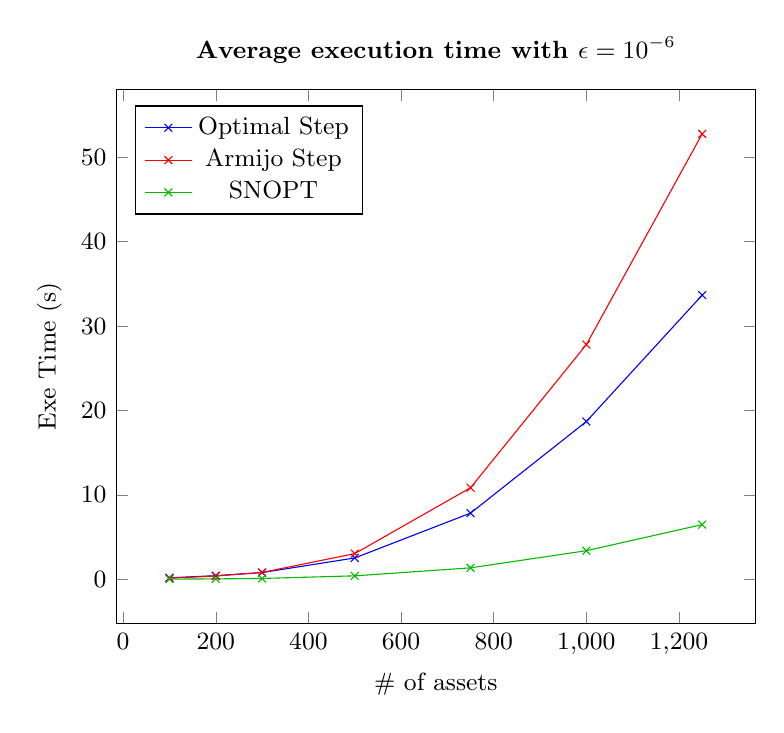
\begin{tikzpicture}
\begin{axis}[%
width=0.8\textwidth,
xlabel={\# of assets},
ylabel={Exe Time (s)},
legend pos=north west,
title=\textbf{Average execution time with {$\epsilon=10^{-6}$}},
]
\addplot [color=blue,solid,mark=x,mark options={solid}]
  table[row sep=crcr]{%
%5	8.3		\\
%10	13.8		\\
%20	25.9		\\
%30	42.5		\\
%50	.088		\\
%75	.141		\\
100	.167	\\
200	.420	\\
300	.787 	\\
500	2.519  	\\
750	7.834		\\
1000 18.686		\\
1250 33.661 \\
%1500 55.57 \\
%2000 197.34 \\
};
\label{Subplot:exe_e6_exact}

\addplot [color=red,solid,mark=x,mark options={solid}]
  table[row sep=crcr]{%
%5	5.5		\\
%10	10.2		\\
%20	19		\\
%30	29.5		\\
%50	.0617		\\
%75	.104		\\
100	.122	\\
200	.374		\\
300	.803		\\
500	3.032	\\
750	10.84		\\
1000	 27.801	\\
1250 52.762\\
};
\label{Subplot:exe_e6_armijo}

\addplot [color=gr,solid,mark=x,mark options={solid}]
  table[row sep=crcr]{%
%5	8.3		\\
%10	13.8		\\
%20	25.9		\\
%30	42.5		\\
%50	.009		\\
%75	.019	\\
100	.010		\\
200	.039		\\
300	.091	\\
500	.399	\\
750	1.347		\\
1000 3.380		\\
1250 	6.470	\\
%2000 32.865 \\
};
\label{Subplot:exe_e8_snopt}
\addlegendentry{Optimal Step}
\addlegendentry{Armijo Step}
\addlegendentry{SNOPT}
\end{axis}
\end{tikzpicture}
}

\makebox[\textwidth][c]{
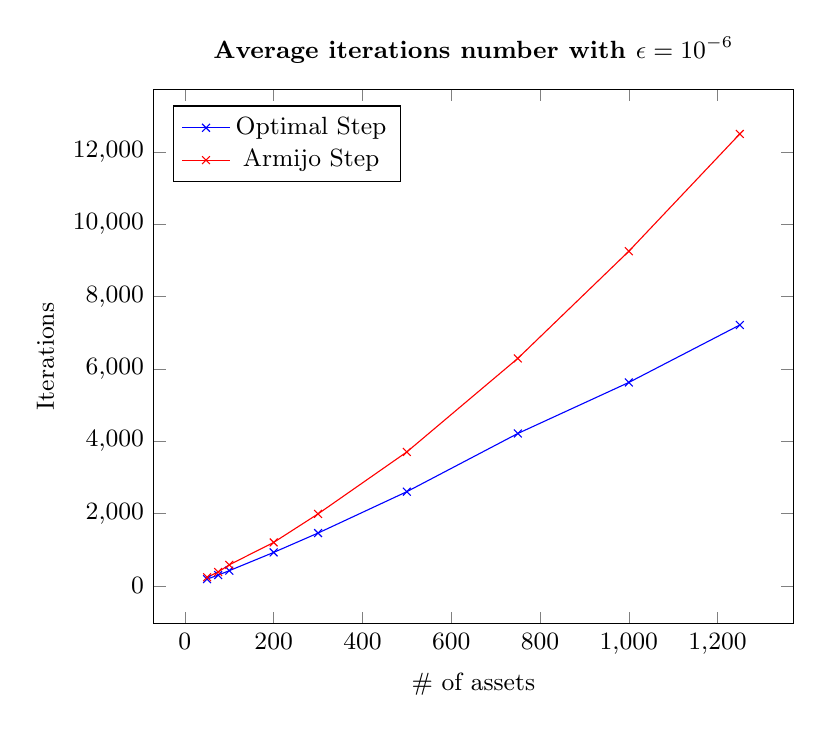
\begin{tikzpicture}
\begin{axis}[%
width=0.8\textwidth,
xlabel={\# of assets},
ylabel={Iterations},
scaled y ticks=false,
legend pos=north west,
title=\textbf{Average iterations number with {$\epsilon=10^{-6}$}}
]
\addplot [color=blue,solid,mark=x,mark options={solid}]
  table[row sep=crcr]{%
%5	22\\
%10	37\\
%20	68\\
%30	105\\
50	188\\
75	300\\
100	422\\
200	927\\
300	1462\\
500	2606\\
750	4215\\
1000	5626\\
1250	7215\\
};
\addplot [color=red,solid,mark=x,mark options={solid}]
  table[row sep=crcr]{%
%5	26		\\
%10	49		\\
%20	92		\\
%30	140		\\
50	240		\\
75	385		\\
100	584		\\
200	1203		\\
300	1992		\\
500	3705		\\
750	6292		\\
1000	9254	\\
1250	12498	\\
};
\addlegendentry{Optimal Step}
\addlegendentry{Armijo Step}
\end{axis}
\end{tikzpicture}
}
\end{figure}

\begin{figure}
\begin{tikzpicture}
\pgfplotsset{every tick label/.append style={font=\small}}
\pgfplotsset{every axis label/.append style={font=\small}}
\begin{axis}[
	ybar stacked,
	title=\textbf{Armijo line search},
    ylabel={\% Exe Time},
    xlabel={\# of assets},
    bar width = 18pt,
    width=0.8\textwidth,
    symbolic x coords={5, 10, 50, 100, 200, 300, 500, 1000},
    xtick=data,
    axis x line*=bottom,
    axis y line*=left,
    area legend,
    legend style={
    legend columns=5,
        at={(xticklabel cs:0.5)},
        anchor=north,
        draw=none
    }
    ]
\addplot[ybar, fill=step] plot coordinates {(5,52) (10,50) 
  (50,47) (100,42) (200,35) (300,27) (500,10) (1000,4)};
\addplot[ybar, fill=derivative] plot coordinates {(5,19) (10,19)(50,23) (100,29) (200,42) (300,57) (500,83) (1000,94)};
\addplot[ybar, fill=theta] plot coordinates {(5,12) (10,13) (50,13) (100,12) (200,10) (300,7) (500,2) (1000,1)};
\addplot[ybar, fill=violation] plot coordinates {(5,14) (10,13) (50,13) (100,13) (200,10) (300,8) (500,4) (1000,1)};
\addplot[ybar, fill=other] plot coordinates{(5,3) (10,5) (50,4) (100,4) (200,3) (300,1) (500,1)};
%\addlegendentry{Step}
%\addlegendentry{Gradient}
%\addlegendentry{Theta}
%\addlegendentry{Most Violating Pair}
%\addlegendentry{Others}
\end{axis}

\end{tikzpicture}

\begin{tikzpicture}
\pgfplotsset{every tick label/.append style={font=\small}}
\pgfplotsset{every axis label/.append style={font=\small}}
\begin{axis}[
    ybar stacked,
    title=\textbf{Optimal step computation},
    ylabel={\% Exe Time},
    xlabel={\# of assets},
    bar width = 18pt,
    width=0.8\textwidth,
    symbolic x coords={5, 10, 50, 100, 200, 300, 500, 1000},
    xtick=data,
    axis x line*=bottom,
    axis y line*=left,
    area legend,
    legend style={
    legend columns=5,
        at={(xticklabel cs:0.5)},
        anchor=north,
        draw=none
    }
    ]
\addplot[ybar, fill=step] plot coordinates {(5,73) (10,73) 
  (50,71) (100,67) (200,58) (300,48) (500,22) (1000,8)};
\addplot[ybar, fill=derivative] plot coordinates {(5,11) (10,10) (50,12) (100,17) (200,27) (300,40) (500,72) (1000,89)};
\addplot[ybar, fill=theta] plot coordinates {(5,7) (10,7) (50,7) (100,7) (200,6) (300,5) (500,2) (1000,1)};
\addplot[ybar, fill=violation] plot coordinates {(5,7) (10,7) (50,7) (100,7) (200,7) (300,6) (500,3) (1000,2)};
\addplot[ybar, fill=other] plot coordinates{(5,2) (10,3) (50,3) (100,2) (200,2) (300,1) (500,1)};
\addlegendentry{Step}
\addlegendentry{Gradient}
\addlegendentry{Theta}
\addlegendentry{Most Violating Pair}
\addlegendentry{Others}
\end{axis}
\end{tikzpicture}
\end{figure}

\clearpage
%% The Appendices part is started with the command \appendix;
%% appendix sections are then done as normal sections
%% \appendix

%% \section{}
%% \label{}

%% If you have bibdatabase file and want bibtex to generate the
%% bibitems, please use
%%
%%  \bibliographystyle{elsarticle-num} 
%%  \bibliography{<your bibdatabase>}

%% else use the following coding to input the bibitems directly in the
%% TeX file.

\begin{thebibliography}{00}
\section{Bibliography}
\bibitem{bai}
  	X. Bai, K. Scheinberg,
  	\emph{Alternating direction methods for non convex
  	optimization with applications to second-order
 	least-squares and risk parity portfolio selection},
  	2015.

\bibitem{snopt}
	P. E. Gill, W. Murray, M. A. Sanders,
	\emph{SNOPT: An SQP Algorithm for large-scale constrained optimization}, 
	2005.


\end{thebibliography}
\end{document}
\endinput
%%
%% End of file `elsarticle-template-num.tex'.
